\chapter{Marco Teórico}

\par En este capítulo se presenta un resumen de los conceptos teóricos, modelos matemáticos y algoritmos necesarios para comprender el desarrollo del trabajo y realizar los cálculos que se usaran luego en la sección de metodología.

\par En primer lugar se da una definición de horno de proceso, se explican los tipos de hornos y las secciones generales que componen estos hornos. Luego se describen los métodos de resolución de ecuaciones utilizados. Por último, se elabora sobre las ecuaciones necesarias para simular los fenómenos en cada sección del horno.

\section{Hornos}

\par Un horno de proceso es un equipo constituido por un cerramiento metálico revestido interiormente por una pared refractaria aislante, dentro del cual se dispone de un serpentín tubular por el que circula un producto que se desea calentar y/o evaporar a través del calor liberado por un combustible sólido, líquido o gaseoso que reacciona en el quemador liberando gases de combustión calientes que entregan calor por radiación al serpentín.

\par Un mazo tubular ubicado por encima de de la zona radiante, en el camino de salida de los gases a la chimenea, recupera calor de los humos, mediante un mecanismo de convección. Esta sección se denomina zona convectiva.

\par La utilización de estos equipos puede tener distintos propósitos como precalentamiento de una corriente previo a su fraccionamiento o reacción, evaporar la corriente de fondo de una columna de destilación o disminuir la viscosidad de un fluido para facilitar su manipuleo.
Pueden utilizarse también como reactores, en este caso proveen el calor de reacción. La cantidad de combustible alimentado al horno se regula normalmente en función de la temperatura de salida de la corriente de proceso.

\par Pueden ser considerados intercambiadores de calor en los que el fluido de proceso fluye dentro de tubos y se calienta por radiación procedente de una llama de combustión y por convección desde los gases calientes de esta.

\par Los hornos son definidos en función de su capacidad de suministro de calor (Duty), medida en millones de Kcal/hora o en millones de Btu/hora. Para la mayoría de los hornos instalados en la industria petrolera, la capacidad suele oscilar entre 10 y 350 MM de Btu/hr. [1]

\section{Tipos de hornos}

\par Los hornos son clasificados dependiendo de su diseño mecánico, como se puede apreciar en la Figura \ref{fig:hornos_tipos} las seis clasificaciones b\'asicas son las siguientes:

\begin{enumerate}[label=\Alph*]
    \item .-  Hornos tipo cabina con serpentín albor.
    \item .-  Hornos tipo cilíndrico con serpentín helicoidal.
    \item .-  Hornos tipo cabina con serpentín horizontal.
    \item .-  Hornos tipo cabina doble con serpentines verticales.
    \item .-  Hornos tipo cilíndrico con serpentines verticales.
    \item .-  Hornos tipo cabina doble con serpentines horizontales.
\end{enumerate}

\begin{figure}[hbt]
\begin{center}
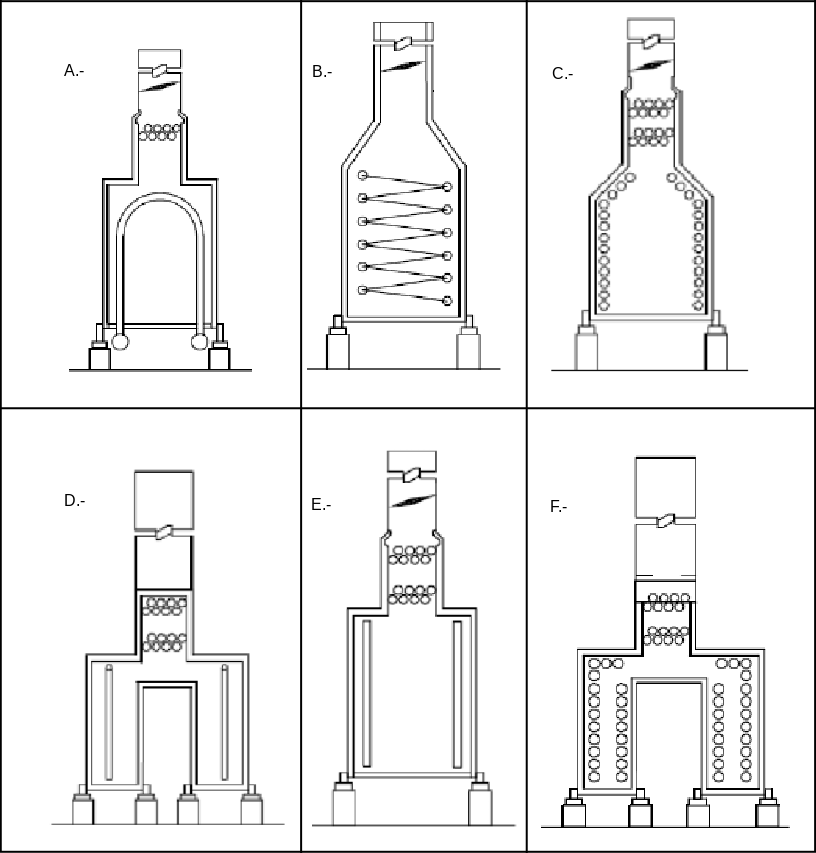
\includegraphics[scale=0.45]{images/hornos_tipos}
\caption[Tipos de hornos por diseño mecánico]{Clasificación de de hornos según su diseño mecánico.}
\label{fig:hornos_tipos}
\end{center}
\end{figure}

\par El horno escogido para simular en este proyecto ha sido uno de tipo cabina con serpentín horizontal, descrito en la Figura \ref{fig:diagrama-meca} y tomado de referencia un horno real ubicado en una refinería de Venezuela.

\begin{figure}[hbt]
\begin{center}
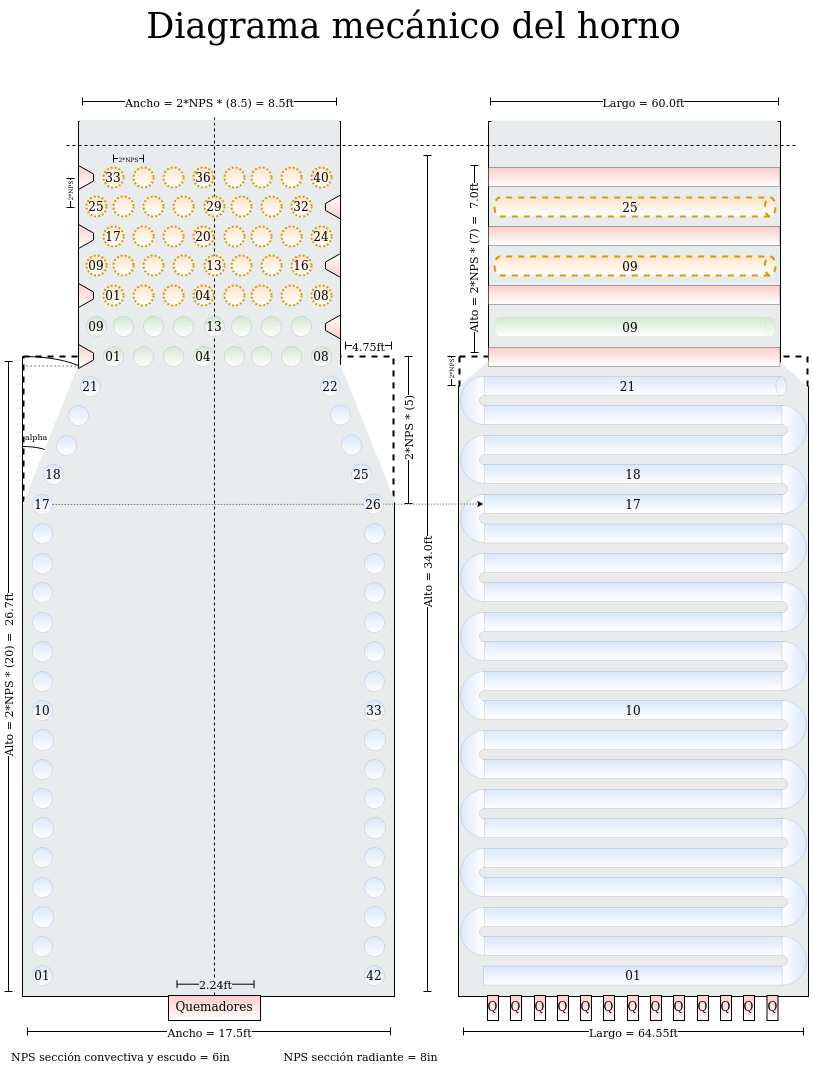
\includegraphics[scale=0.38]{images/diagrama-meca}
\caption[Diagrama mecánico]{Diagrama mecánico del horno simulado.}
\label{fig:diagrama-meca}
\end{center}
\end{figure}

\section{Combustión}
\par De este fenómeno se produce todo el calor usado por el horno para transferir a el fluido ingresado. Este calor proviene de la reacción química de combustión del combustible seleccionado para el proceso.

\par La combustión se da físicamente encima de los quemadores, espacio donde se mezcla el combustible con el comburente, \ac{o2}, normalmente extraído de una corriente de aire ambiental, cuya composición se aproxima a 20.95\% de \ac{o2} y 79.05\% de \ac{n2} para los cálculos necesarios. Como ejemplo de esta reacción balanceada se puede observar la ecuación \ref{eq:combustion}, donde se usa \ac{ch4} como combustible, los moles de \ac{n2} provienen de la relación volumétrica entre los compuestos del aire teórico 79.05/20.95 = 3.76.

\begin{equation}
    \label{eq:combustion}
    CH_4 + 2O_2 + 2(3.76)N_2 \rightarrow CO_2 + 2H_2O + 7.52N_2
\end{equation}

\par La mínima cantidad de aire que puede suministrar \ac{o2} suficiente para una reacción completa es llamado aire teórico. En la practica, la combustión completa no sera lograda a menos que el aire suministrado sea mayor al 100\% del aire teórico y empieza a ser llamado exceso de aire.

\par Un parámetro importante, usualmente usado para expresar la relación de aire y combustible es la relación aire/combustible (designada como AC, ec. \ref{eq:ac}). Usualmente expresada en base másica, pero puedo encontrarse en base molar, como se muestra en la ecuación \ref{eq:ac}

\begin{gather}
    \label{eq:ac}
    AC_{masa} = \frac{m_{aire}}{m_{combustible}}\\
    AC_{molar} = \frac{n_{aire}}{n_{combustible}}
\end{gather}

\par Y se relacionan a través de la masa molar:

\begin{equation}
    AC_{masa} = \frac{m_{aire}}{m_{combustible}} =
    \frac{n_{aire}*M_{aire}}{n_{combustible}*M_{*M_{aire}}} = AC_{molar}*\frac{M_{aire}}{M_{M_{aire}}}
\end{equation}

\par Requerido en los siguientes pasos del desarrollo, de la reacción de combustión se obtiene el \ac{ncv}, valor crucial para el cálculo del calor suministrado por el combustible al horno. Para profundizar en este tema y observar las ecuaciones de \ac{cp}, entalpía y energía interna de combustión usadas se recomienda acudir al texto de fundamentos de termodinámica\cite{bib:vanwylen}, capítulo 15, nombrado en las referencias.

\par Luego de definir estos aspectos se puede plantear un balance de energía global, usando el horno como volumen de control, ec. \ref{eq:balance-global}, donde se aprecia la distribución del calor generado en la combustión. Ver la Figura \ref{fig:balance-energic}.

\begin{figure}[hbt]
\begin{center}
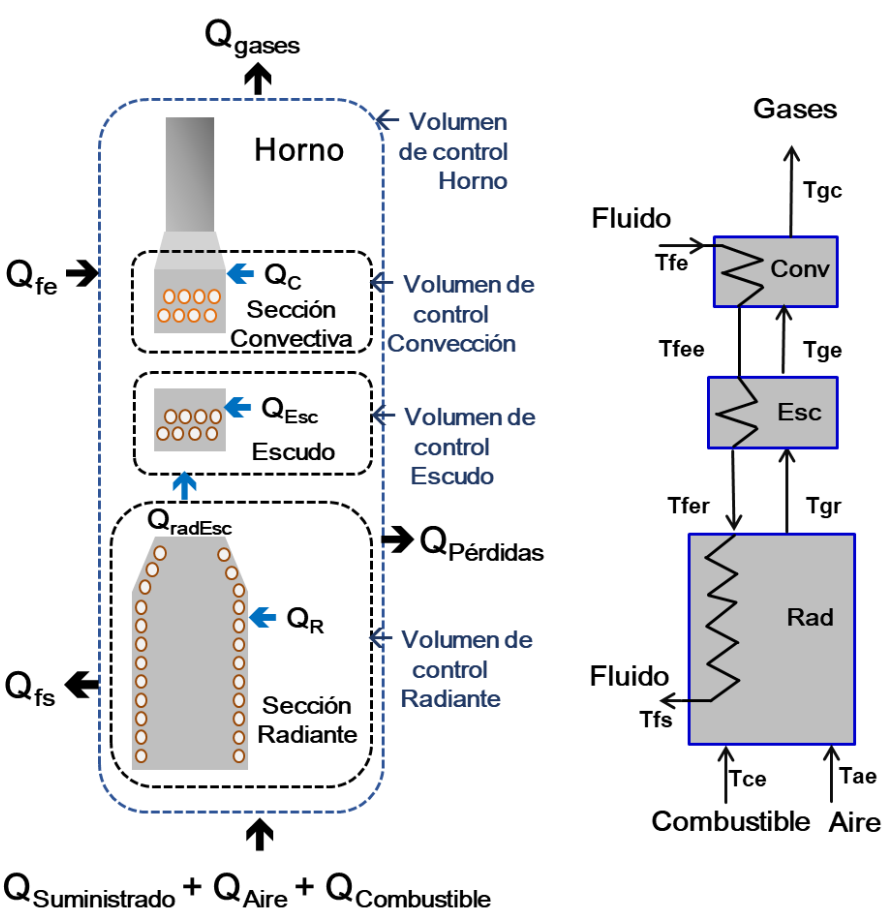
\includegraphics[scale=0.38]{images/balance-energic}
\caption[Balance de energía del horno]{Balance global de energía en el horno y similitud con intercambiador de tres etapas.}
\label{fig:balance-energic}
\end{center}
\end{figure}

\begin{equation}
    \label{eq:balance-global}
    \begin{gathered}
    Q_{entrada} = Q_{salida}\\
    Q_{suministrado} + Q_{aire} + Q_{combustible} + Q_{f_{entrada}} = 
    Q_{gases} + Q_{f_{salida}} + Q_{perdidas}
    \end{gathered}
\end{equation}

donde:\\
$Q_{suministrado} = NCV * m_{combustible}$\\
$Q_{perdidas} = Calor perdido por falta de hermeticidad$\\
$Q_{otros compuestos} = m_{otros compuestos} * Cp_{otros compuestos}(T) * \Delta T$

\section{Zonas y balances de energía en el horno}

\par El horno puede ser dividido en zonas o secciones para simplificar los cálculos, como se pudo apreciar en la sección de tipos de horno, el arreglo mecánico puede variar pero para fines de este análisis se ha dividido el horno en tres zonas o volúmenes de control: radiativa, escudo y convectiva. El volumen de control radiativo corresponde a la sección radiante (o también llamada de radiación) del horno, y los volúmenes de control escudo y convectivo forman parte de una misma sección del horno, la sección convectiva. La división de la sección convectiva es debida a que las dos zonas presentan diferencias en los mecanismos de transferencia de calor, así, los tubos de la zona escudo reciben radiación luminosa directa de la llama,  la cual no está presente en la zona convectiva. La zona escudo está formada por las dos o tres primeras filas de tubos de la sección convectiva y son tubos lisos, mientras que la zona convectiva está formada generalmente por tubos con aletas. En ambas zonas está presenta la radiación del gas y la reflectada de las paredes de la sección hacia los tubos. Esta radiación, de baja longitud de onda, deja de ser significativa por debajo de los 550 C (1000 F).
 
\par Conociendo que la energía transferida al fluido de proceso es igual a

\begin{equation}
    \begin{gathered}
    Q_{fs} - Q_{fe} = Q_{RAD} + Q_{ESC} + Q_{CONV}\\
               	    = m_f * C_p * (T_{fs} - T_{fe})
    \end{gathered}
\end{equation}

\par Donde $Q_{RAD}, Q_{ESC}, Q_{CONV}$ son el calor que transfiere el gas de combustión al fluido en las zonas radiante, de escudo y convectiva respectivamente y que corresponde al servicio (duty) del horno, substituyendo en ecuación \ref{eq:balance-global}.

\begin{equation}
    Q_{suministrado} + Q_{aire} + Q_{combustible} = Q_{RAD} + Q_{ESC} + Q_{CONV} + Q_{perdidas} + Q_{gases}
\end{equation}

\par La incógnita se reduce a cuantificar $Q_{RAD}, Q_{ESC}, Q_{CONV}, Q_{perdidas}$ y la temperatura de salida de los gases con el objetivo de:
\begin{enumerate}
    \item Dimensionar el horno para un determinado servicio o duty, y calcular la cantidad de combustible requerido, $Q_{suministrado}$.
    \item Calcular el comportamiento del horno ante variaciones de las condiciones operacionales, tales como, cambios en la composición de combustible, en la relación aire-combustible, el flujo del fluido de proceso, el requerimiento de temperatura de salida del fluido, etc.
\end{enumerate}

\subsection{Zona Radiante}
\par Es donde los tubos que trasportan el fluido de proceso reciben radiación directa desde la llama del quemador y las paredes refractarias. En esta parte la transmisión de calor es por radiación en un 80\% aproximadamente, y un 20\% por convección de la circulación de gases calientes alrededor de los tubos.

\par El análisis descrito a continuación está basado en el modelo presentado inicialmente por (Lobo \& Evans)\cite{bib:rad} y parte de la suposición de un mezclado ideal de los gases producto de la combustión en la sección radiante lo cual implica, en consecuencia, una temperatura uniforme del gas en todo el volumen de la sección radiante, denominada \ac{tg}, la cual será la temperatura efectiva de transferencia de calor entre los gases de combustión y la superficie de los tubos y será igualmente la \ac{tgr} hacia el escudo de tubos.

\par Realizando el balance de energía en el volumen de control de la sección radiante resulta:

\begin{equation}
    \label{eq:rad}
    Q_{suministrado} + Q_{aire} + Q_{combustible} = 
    Q_{RAD} + Q_{radEsc} + Q_{CONV} + Q_{perdidas} + Q_{gases}
\end{equation}

\par En la zona radiante se transfiere calor al fluido por dos mecanismos, mediante radiación directa y por convección entre los gases producto de la combustión y el fluido,

\begin{equation}
    \label{eq:rad-fluid}
    Q_{RAD} = Q_{rad} + Q_{conv} = m_f * C_{p_f} * (T_{fs} - T_{fer})
\end{equation}

\par Donde $Q_{rad}, Q_{conv}$ son el calor que se transfiere al fluido en la sección radiante por radiación y por convección, y $Q_{radEsc}$ es el calor por radiación que se transfiere a los tubos del escudo desde la zona radiante.

\par Usando las siguientes ecuaciones de transferencia de calor:

\begin{equation}
    Q_{rad} = \sigma * ( \alpha * A_{cp} )_{R} * F * ( T_{g}^{4} - T_{w}^{4} )
\end{equation}
$\sigma$ = Constante de Stefan-Boltzman.\\
$\alpha$ = Factor de efectividad relativa del banco de tubos.\\
$A_{cp}$ = Área del plano frontal a la llama del banco de tubos.\\
F = Factor de transferencia radiante.\\
$T_g$ = Temperatura efectiva del gas en la zona radiante (°R o K)\\
$T_w$ = Temperatura promedio de la pared del tubo, (°R o K)

\begin{gather}
    Q_{conv} = h_{conv} * A_t * (T_g - T_w)\\
    Q_{radEsc} = \sigma * ( \alpha * A_{cp} )_{Esc} * F * ( T_{g}^{4} - T_{w}^{4} )
\end{gather}

\par Si se considera que las pérdidas por las paredes del horno equivalen al 1.5\% del calor suministrado (entre 1,5 y 5.0) los calores resultan en:
\begin{gather}
    Q_{suministrado} = NCV * m_{combustible}\\
    Q_{perdidas} = 0.015 * NCV * m_{combustible}\\
    Q_{aire} = m_{aire} * C_{p_A} * (T_A - T_{Ref})\\
    Q_{combustible} = m_{combustible} * C_{p_C} * (T_C - T_{Ref})\\
    Q_{gases} = m_{gases} * C_{p_g} * (T_g - T_{Ref})
\end{gather}

\par Donde $T_{Ref}$ es la temperatura de referencia utilizada para calcular las propiedades termodinámicas (condiciones estándar de presión y temperatura).

\begin{equation}
    m_{gases} = m_{combustible} * AC_{masa} + m_{combustible} = 
    m_{combustible} (1 + AC_{masa})
\end{equation}

Substituyendo  en las ecuaciones (\ref{eq:rad}) y (\ref{eq:rad-fluid}) se obtiene:

\begin{equation}\label{eq:rad-tgr}
\begin{gathered}
    m_C*NCV +m_A*C_{p_A}*(T_A -T_{Ref}) + m_C*C_{p_C}*(T_C -T_{Ref}) = \\
    m_C*(1 +AC_{masa})*C_{p_G}*(T_g -T_{Ref}) + \\
    \sigma *(\alpha *A_{cp})_{Esc}*F*(T_g^4-T_w^4) + \\
    \sigma *(\alpha *A_{cp})_R F (Tg4 - Tw4) + \\
    h_{conv}*A_t*(T_g -T_w) + \\
    0.015*m_C*NCV
\end{gathered}
\end{equation}
\begin{equation}
\label{eq:rad-comp}
Q_R = 
\sigma * (\alpha * A_{cp})_R *F *(T_g^4 -T_w^4) +h_{conv} *A_t *(T_g -T_w)
= m_f * C_{p_f} * (T_{fs} - T_{fer})
\end{equation}
\par La ecuación (\ref{eq:rad-tgr}) permite calcular la \ac{tgr}, o el flujo másico de combustible requerido, $m_C$, mediante un proceso de ensayo-error o en su defecto, utilizando un algoritmo de cálculo numérico (p. ej., el método usado para este desarrollo fue Newton Raphson). La ecuación (\ref{eq:rad-comp}) permite calcular la  temperatura efectiva de llama Tgr a partir de un estimado del calor transferido al fluido en la zona radiante ($Duty_{rad}$).

\subsubsection{Temperatura de pared (Tw)}
\par La temperatura de pared puede ser calculada a partir de la ecuación de transferencia de calor entre el fluido y la pared externa del tubo:
\begin{equation*}
    q_{rad} = Q_R / A_o
\end{equation*}

donde $q_{rad}$ es el flujo de calor por unidad de área exterior del tubo (densidad de flujo de calor) en la zona radiante.
\begin{gather*}
q_{rad} = \frac{(Q_{rad} + Q_{conv})}{A_o} = (T_w - T_b) / (A_t *\Sigma R) \\
\Sigma R = R_{conv} + R_{fi} + R_t
\end{gather*}

\par Que corresponden a la resistencia convectiva interna, el factor de ensuciamiento y la resistencia conductiva de la pared del tubo. Resolviendo por $T_W$
\begin{equation}
\label{eq:tw}
T_W = q_{rad} *(d_o/d_i) *[ R_{fi} + 1/h_i + d_i*ln(d_o/d_i)/(2*k_w) ] +T_b
\end{equation}

\par Donde,\\
$T_b$ es la temperatura de mezcla del fluido $(T_{fs} + T_{fer})/2$. \\
$k_w$ es la conductividad térmica del tubo. \\
$h_i$ es el coeficiente interno de transferencia de calor. \\
$R_{fi}$ es el factor de ensuciamiento interno del tubo. \\

\par Para resolver la ecuación (\ref{eq:tw}) se necesita calcular la temperatura de entrada del fluido a la zona radiante, $T_{fer}$ a partir del estimado hecho de $Q_R$. 

\subsubsection{Coeficiente interno de transferencia de calor (coeficiente de película del fluido)}

\par El coeficiente interno de transferencia de calor es calculado para líquidos por la ampliamente usada ecuación
\begin{equation}
\label{eq:hi}
 h_i = 0.023 * \frac{k_f}{d_i} *Re^{0.8} *Pr^{1/3} *(\mu_b /\mu_w )^{0.14}
\end{equation}
\par Donde,\\
$\mu_b$ y $\mu_w$ son las viscosidades del fluido de proceso a $T_b$ y $T_w$. \\
Re, es el número de Reynolds evaluado a la temperatura $T_b$. \\
Re = $(\rho v d_i / \mu)_b = (G *d_i / \mu)_b$. \\
G, es el flujo másico por unidad de área. \\
Pr, es el número de Prandtl del fluido de proceso. \\
Pr = $(\mu C_p / k)_f$ evaluado a $T_b$.

\subsubsection{Coeficiente convectivo de la zona radiante}

\par El coeficiente convectivo de la parte exterior de los tubos en la zona convectiva, para un horno tipo cabina con tubos en la pared ha sido estimado en
\begin{equation}
h_{conv} = 1.5  BTU/(hr ft^2 F) \approx 8.5 W/(m^2 C)
\end{equation}

Con esta última ecuación quedan definidos todos los términos de las ecuaciones (\ref{eq:rad-tgr}) y (\ref{eq:rad-comp}).

\subsubsection{Factor de eficiencia del banco de tubos ($\alpha$)}

Factor de eficiencia, $\alpha$, debido a que el banco de tubos no absorbe todo el calor radiado al plano frío, un factor de eficiencia de absorción puede ser usado para corregir esta área y dependerá del arreglo de tubos. El factor de eficiencia relativa se describe bajo las siguientes curvas:
\par Para una fila de tubos simple frente a la pared refractaria, usar (Total One Row). Para dos filas de tubos frente a la pared refractaria, usar (Total Two Rows). Para hornos de doble llama, usar (Direct OneRow). Ver la Figura \ref{fig:alpha}.

\begin{figure}[hbt]
\begin{center}
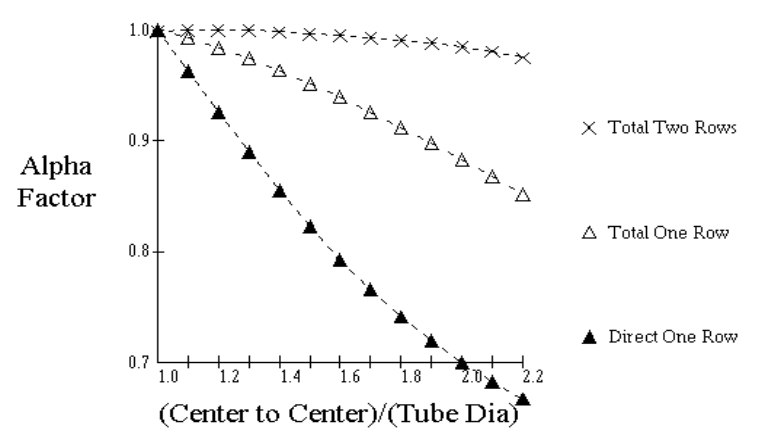
\includegraphics[scale=0.45]{images/alpha}
\caption[Eficiencia de absorción para banco de tubos]{Eficiencia de absorción para banco de tubos.}
\label{fig:alpha}
\end{center}
\end{figure}

\subsubsection{\ac{acp}}

\par Las superficies normales de absorción de calor en un horno consisten en una serie de tubos paralelos. En el caso de un diseño de hornos donde los tubos se reciben la llama desde un solo lado, los tubos normalmente se colocan frente a una pared refractaria. Parte de la radiación del gas caliente incide directamente en los tubos, mientras que el resto pasa a través y se irradia de regreso a la cámara, donde parte es absorbida por los tubos por refracción. En el caso de tubos expuestos desde ambos lados, por ejemplo, cuando los tubos están colocados en el centro de la cámara, los tubos absorben la radiación directa desde ambos lados. Expresar el área del tubo como un área plana equivalente simplifica este cálculo. El área de plano frío calculada es el área de un plano a través de las líneas centrales del tubo, ya sea que estén en un plano curvo, como en un patrón cilíndrico o en una fila de lado a lado. Para la mayoría de los paneles de tubos, el ancho sería igual al espacio centro/centro de los tubos multiplicado por el número de tubos. La longitud efectiva es la longitud del tubo expuesto a la radiación. En el caso de tubos que penetran en una placa tubular, es la longitud entre placas tubulares. Pero para los tubos con las curvas de retorno dentro de la cámara de combustión, la longitud puede tomarse como la distancia desde la línea central del retorno en un extremo hasta la línea central del retorno en el otro extremo.

\par Para una cámara de combustión con los tubos hacia abajo en el centro, u otro patrón que resulte en que los tubos se disparen desde ambos lados, el área del plano frío sería el doble del área proyectada.

\par Para llama de un solo lado:
\begin{equation}
Acp = N_{tubo} * S_{tubo} * L_{tubo}
\end{equation}
\par Para llama de ambos lados:
\begin{equation*}
Acp = N_{tubo} * S_{tubo} * L_{tubo} * 2
\end{equation*}
\par Donde, \\
$N_{tubo}$ = Número de tubos. \\
$S_{tubo}$ = Espaciado de tubos. \\
$L_{tubo}$ = Largo efectivo del tubo.

\subsubsection{Factor global de transferencia radiante (F)}
\par Debido a que el gas de combustión en el horno es un mal medio de radiación, la ecuación debe ser corregida usando un factor de transferencia radiante dependiente de la emisividad del gas y la relación del área refractaria de plano frío. Como el calor de radiación es reflejado de regreso al horno, por refracción, un horno con mayor relación de de superficie refractaria con respecto a la superficie de los tubos, absorberá mas calor. Como los tubos no absorben perfectamente el calor, las curvas esta basadas en superficies de tubos con absorción de 0.9. Un valor considerado como típico para superficies de metales oxidados. El factor de transferencia radiante final puede ser tomado de la siguiente curva (Figura \ref{fig:f}) ofrecida por Mekler \& Fairall\cite{bib:mekler}.

\begin{figure}[hbt]
\begin{center}
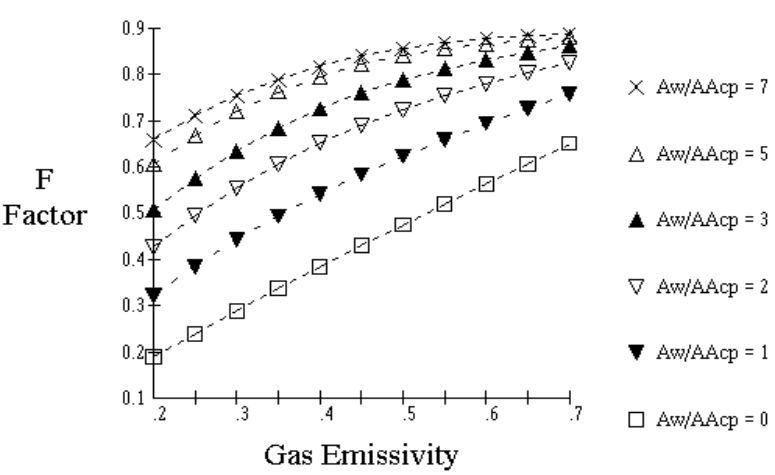
\includegraphics[scale=0.45]{images/f}
\caption[Factor de transferencia radiante, F]{Factor de transferencia radiante, F.}
\label{fig:f}
\end{center}
\end{figure}

\par Donde $Aw$/$\alpha$Acp es calculada con la ecuación \ref{eq:aw-acp}. El área de plano frío equivalente, $\alpha$Acp, es el producto del factor de efectividad y del área de plano frío como se describió anteriormente. Área refractaria efectiva se calcula con:

\begin{equation}
Aw = Ar - \alpha Acp
\end{equation}

\par El área refractaria total, Ar, es el total del área refractaria expuesta a la sección radiante del horno. Cuando hay sección de escudo, que recibe radiación directa, el $\alpha$Acp para la sección radiante y para la sección de escudo se calculan de forma independiente y luego son sumados para calcular el factor de transferencia radiante.

\par La ecuación para $Aw$ se convierte en:
\begin{equation}
Aw = Ar - ((\alpha Acp)_{rad} + (\alpha Acp)_{esc})   
\end{equation}

\par Para finalmente:

\begin{equation}
\label{eq:aw-acp}
Aw/\alpha Acp = \frac{Aw}{(\alpha Acp)_{rad} + (\alpha Acp)_{esc}}
\end{equation}
 
\subsubsection{Emisividad de gases de combustión}
\par La emisividad de un gas puede ser descrita por la curva presentada por Lobo y Evans\cite{bib:rad}, la temperatura de pared tiene solo un efecto menor. Por lo tanto, la emisividad puede ser correlacionada como una función del PL (\ref{eq:pl}) producido y la temperatura del gas de combustión, Tg. Variaciones en la temperatura de pared entre 600ªF y 1200 ªF causan una desviación menor al 1\% de estas curvas.

\begin{figure}[hbt]
\begin{center}
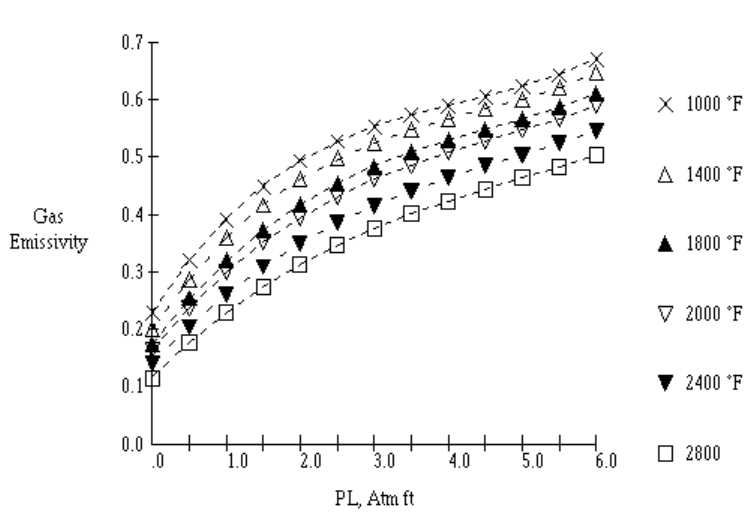
\includegraphics[scale=0.45]{images/emiss}
\caption[Emisividad del gas]{Emisividad del gas.}
\label{fig:emiss}
\end{center}
\end{figure}

\begin{equation}
\label{eq:pl}
PL = (PH_2O + PCO_2) * MBL
\end{equation}

\par Donde $PH_2O$ y $PCO_2$ son las presiones parciales del \ac{h2o} y \ac{co2} en el gas, y MBL en pies obtenido de la tabla \ref{tbl:mbl}.

\subsubsection{\ac{mbl}}
\par Para el cálculo de la \ac{mbl}, la distribución de los tubos debe ser tomada en cuenta. Si el horno es de forma rectangular con tubos en el centro, la \ac{mbl} será la mitad del área rectangular del horno. Longitudes del láser para otras configuraciones, como un horno cilíndrico con una disposición de tubos octagonal o tubos cruzados, deberá ser calculada con esas consideraciones.

\par La \ac{mbl} para hornos puede ser tomada, de acuerdo a Wimpress\cite{bib:wimpress} como se muestra en la Tabla \ref{tbl:mbl}.:

\begin{table}
\caption[Calculo del MBL]{Cálculo del MBL con dependencia de las dimensiones de la cámara de combustión}
\label{tbl:mbl}
    \centering
    \begin{tabular}{c|c}
        Relación de dimensión  & Longitud de láser media \\
        \hline
        1-1-1 a 1-1-3   & \multirow{2}{10em}{2/3 * (Vol. horno)$^{1/3}$} \\
        1-2-1 a 1-2-4   & \\
        \hline
        1-1-4 a 1-1-inf & 1 * Menor dimensión \\
        \hline
        1-2-5 a 1-2-inf   & 1.3 * Menor dimensión \\
        \hline
        1-3-3 a 1-inf-inf & 1.8 * Menor dimensión \\
        \hline
        \multicolumn{2}{c}{Para hornos cilíndricos verticales} \\
        \hline
        Largo/Diámetro $<$ 2  & (($\frac{L}{D}$-1)*0.33 + 0.67)*D\\
        \hline
        Largo/Diámetro $\geq$ 2 & Diámetro\\
    \end{tabular}
    \caption{MBL para hornos rectangulares}
    \label{tbl:mbl}
\end{table}

\subsection{Zona Escudo}
\par Esta zona contiene las primeras filas de tubos del área de convección que "protegen" (\textit{shield}) el resto de la zona de convección, en ella los tubos no tienen aletas y reciben la misma cantidad de calor por ambos mecanismos.

\par Según  han reportado  Mekler \& Fairall\cite{bib:mekler}  la radiación luminosa desde la sección radiante a los tubos de la zona escudo, $Q_{radEsc}$ puede ser repartida un 76.92\% en la primera fila y el 23.08\% restante en la segunda fila. Esta aproximación conjuntamente con la distribución circular del flujo de calor es usada para calcular la temperatura máxima de pared en los tubos de la zona de escudo.

\par Realizando un balance de energía en la zona de los tubos de escudo

\begin{equation}
\label{eq:esc}
Q_{entradaEsc} = Q_{fe} + Q_{gas-e} + Q_{radEsc} = 
Q_{fs} + Q_{gas-s} = Q_{salidaEsc}
\end{equation}

\par Donde $Q_{radEsc}$ es el calor por radiación que escapa desde la zona radiante hacia el escudo de tubos y que ya ha sido calculado al determinar la temperatura efectiva de radiación Tg. La temperatura de entrada del gas a la zona de escudo Tgr es igual a la temperatura efectiva Tg, lo cual se infiere de haber supuesto una temperatura de mezcla ideal de los gases en la sección radiante. $Tgr = Tg$

\par Rearreglando la ecuación \ref{eq:esc}, se obtiene:
\begin{equation*}
Q_{fs} - Q_{fe} = Q_{gas-e} - Q_{gas-s} + Q_{radEsc} = Q_{Esc}
\end{equation*}
\par Donde,
\begin{equation}
\label{eq:qesc}
m_{f} *C_{p_f} *(T_{fer} - T_{fee}) = 
m_{g} *C_{p_g} *(T_{gr}  - T_{ge}) + Q_{radEsc} = Q_{Esc}
\end{equation}
\begin{equation}
Q_{radEsc} = \sigma *(\alpha *A_{cp} )_{Esc} *F *(T_{gr}^4 -T_w^4)
\end{equation}

\par Para los gases el cambio de entalpía dentro de zona del escudo se debe a la transferencia de calor hacia los tubos.
\begin{equation}
\label{eq:qesc-lmtd}
m_{g} *C_{p_g} *(T_{gr} -T_{ge}) = Uo *Ao *LMTD
\end{equation}

\par Donde LMTD es la Diferencia de Temperatura Media Logarítmica entre el gas de combustión y el fluido del proceso, expresada por:
\begin{equation}
\label{eq:lmtd}
   LMTD = \frac{(T_{gr}-T_{fer}) - (T_{ge}-T_{fee})}
   {ln[(T_{gr}-T_{fer}) /(T_{ge}-T_{fee})]}
\end{equation}
Sustituyendo (\ref{eq:qesc-lmtd}) en (\ref{eq:qesc})
\begin{equation}
\label{eq:tesc}
  Q_{Esc} = m_{f} *C_{p_f} *(T_{fer} - T_{fee}) = Uo *Ao *LMTD + Q_{radEsc}
\end{equation}

\subsubsection{Coeficiente Global de Transferencia de Calor en el Escudo}

\par Generalmente el escudo de tubos está formado por dos o tres filas de tubos lisos (sin aletas) pero formando parte del banco de tubos de la sección superior del horno que incluye otra zona de tubos aletados, para un banco de tubos lisos el coeficiente global de transferencia de calor viene dado por la ecuación:
\begin{gather*}
\label{}
Uo  = 1 / \Sigma R \\
\Sigma R = R_o + R_t + R_i
\end{gather*}

\par Donde $R_o, R_t, R_i$ son la resistencia externa de la pared del tubo, la resistencia interna del tubo y el factor de ensuciamiento interno respectivamente.
\par Sustituyendo:
\begin{equation}
\label{}
\Sigma R = \frac{1}{h_o} +\frac{d_o*ln(d_o/d_i)}{2*k_t} +\frac{A_o}{A_i*h_i} +R_{fi}
\end{equation}

\begin{equation}
\label{}
m_{g} *C_{p_g} *(T_{gr} - T_{ge}) = \frac{Ao *LMTD}
{\frac{1}{h_o} +\frac{d_o*ln(d_o/d_i)}{2*k_t} +\frac{d_o}{d_i*h_i} +\frac{d_o}{d_i}R_{fi}}
\end{equation}

\par Donde el coeficiente interno de película se calcula como en el caso de los tubos de la sección radiante mediante la ecuación \ref{eq:hi}:

\par El coeficiente externo $h_o$ puede ser expresado como la sumatoria de las resistencias externas como:
\begin{equation}
\label{eq:ho}
h_o = 1/(\frac{1}{h_c + h_{re}} + R_{fo})
\end{equation}
\par Donde \\
$h_c$ es el coeficiente de película externo.\\
$h_r$ es el coeficiente efectivo de radiación hacia la pared del tubo.\\
$R_{fo}$ es el factor de ensuciamiento externo.\\

\par El coeficiente de película exterior para un banco de tubos lisos colocados triangularmente (tresbolillo) puede ser calculado por:
\begin{equation}
\label{eq:hc}
\begin{gathered}
h_c = 0.33 * \frac{k_{gb}}{d_o} *Pr_{gb}^{1/3} *Re_{gb}^{0.6}\\
h_c = 0.33 * \frac{k_{gb}}{d_o} *Pr_{gb}^{1/3} *(\frac{d_o*G_n}{\mu_{gb}})^{0.6}
\end{gathered}
\end{equation}
$G_n$ es la velocidad másica basada en el área libre para el flujo de gas, es decir, el espacio entre los tubos por el largo del horno.

\par El coeficiente efectivo de radiación se refiere al calor por radiación que transfiere el gas de combustión más el calor reradiado de las paredes de la zona de escudo a la pared de los tubos. Como aproximación el coeficiente de radiación para la zona de escudo y convectiva puede ser obtenido de la siguiente ecuación empírica:
\begin{equation}
\label{eq:hr}
h_r = 0.092*T_g - 34  
\end{equation}
\par Donde Tg es la temperatura del gas en °K y $h_r$ viene expresado en kJ/m$^2$h°K

\par Otro método para el cálculo de $h_{re}$ se tratará más adelante, conjuntamente con el de la zona convectiva.

\subsubsection{Coeficiente efectivo de absorción de radiación. Tubos escudo}
\par Dado que todo el calor dirigido hacia este banco de tubos sale de la sección radiante y es absorbido por los tubos, el factor de efectividad de absorción relativa, $\alpha$, para los tubos de escudo puede tomarse igual a uno.

\subsubsection{Cold Plane Area, Acp. Tubos escudo}
\par El área de plano frío para la sección de escudo es igual al área de plano frío de la primera fila de tubos de esta sección.
\begin{equation*}
Acp = N_tubo * S_tubo * L_tubo
\end{equation*}
\par Donde, \\
$N_{tubo}$ = Número de tubos por fila. \\
$S_{tubo}$ = Espaciado de tubos. \\
$L_{tubo}$ = Largo efectivo del tubo.\\

\par Los valores usados para el factor de intercambio, F, temperatura efectiva del gas en la cámara de radiación, Tgr, y temperatura de pared promedio, Tw, son los mismos valores usados en la sección radiante.

\subsection{Zona Convectiva}
\par En esta zona el calor del gas hacia los tubos se transfiere en forma similar al de la zona escudo. En el lado exterior de los tubos se trasfiere calor por radiación y por convección en paralelo, pero en este caso la presencia de las aletas modifica el cálculo de los coeficientes de transferencia de calor.

\par El balance de energía depende de la energía entrando y saliendo del gas y del fluido del proceso resulta en:

\begin{equation}
\label{eq:conv}
Q_{entrada} = Q_{fe} + Q_{gas-e} = Q_{fee} + Q_{gas-s} = Q_{salida}
\end{equation}

\par Rearreglando:
\begin{equation*}
Q_{fee} - Q_{fe} = Q_{gas-e} - Q_{gas-s} = Q_{CONV}
\end{equation*}
\begin{equation}
\label{eq:qconv}
m_{f} *C_{p_f} *(T_{fer} - T_{fee}) = 
m_{g} *C_{p_g} *(T_{ge}  - T_{gc}) = Q_{CONV}
\end{equation}
\par Los valores de $C_{p_f}$ y $C_{p_g}$ son calculados a la temperatura promedio del fluido y del gas.

\subsubsection{Transferencia convectiva, tubos aletados}
\par Las ecuaciones de transferencia de calor para los tubos con aletas son básicamente las mismas que para los tubos desnudos hasta que llega al factor $h_e$, donde se introduce un nuevo concepto para explicar la aleta o superficie extendida.

\subsubsection{Coeficiente global de transferencia de calor, Uo}

\begin{equation}
Q_{CONV} = Uo *Ao *LMTD
\end{equation}

\begin{gather*}
\label{}
Uo  = 1 / \Sigma R \\
\Sigma R = R_o + R_t + R_i \\
\Sigma R =  \frac{1}{h_{oe}} 
            +\frac{d_o*ln(d_o/d_i)}{2*k_t} 
            +(\frac{1}{h_i}+R_{fi})*\frac{d_o}{d_i} 
\end{gather*}

\subsubsection{Coeficiente externo efectivo de transferencia de calor, $h_{oe}$}
\begin{equation*}
h_{oe} = h_o * (E *Afo +Apo) / Ao
\end{equation*}

\par Donde,\\
E = Eficiencia de las aletas\\
Ao = Área de superficie externa total.\\
Afo = Área de superficie externa de aletas. \\
Apo = Área de superficie de tubos. \\

\par Y, $h_o$, coeficiente externo promedio de transferencia de calor: 
\begin{equation*}
h_o = 1/(\frac{1}{h_c+h_r}+R_{fo})
\end{equation*}

\par Donde,\\
$h_r$ = Coeficiente externo de radiación de transferencia de calor.\\
$R_{fo}$ = Resistencia de ensuciamiento externo. \\

\par Y, $h_c$, coeficiente de película externo de transferencia de calor: 
\begin{equation*}
h_c = j *G_n *C_{p_g} *(Pr_g)^{0.67}
\end{equation*}

\par Donde,\\
j = Factor Colburn de transferencia de calor.\\
$G_n$ = Velocidad másica basada en el área libre neta.\\
$Pr_g$ = Número de Prandtl del gas $(\mu*C_p /k)_{gb}$ evaluado a $T_{gb}$.\\
$C_{p_g}$ = Capacidad calorífica del gas.\\
$k_b$ = Conductividad térmica del gas.\\
$\mu_b$ = Viscosidad dinámica del gas.\\

\subsubsection{Factor Colburn de transferencia de calor, j}
\begin{equation*}
j = C_1 *C_3 *C_5 *(\dfrac{d_f}{d_o})^{0.5} *(\frac{T_b}{T_s})^{0.25}
\end{equation*}

\par Donde, \\
$C_1$ = Corrección del número de Reynolds. \\
$C_3$ = Corrección geométrica. \\
$C_5$ = Corrección no-equilateral y de fila. \\
$d_f$ = Diámetro externo de la aleta. \\
$d_o$ = Diámetro externo del tubo. \\
$T_b$ = Temperatura promedio del gas, K. \\
$T_s$ = Temperatura promedio de aleta, K.\\

\par Corrección del número de Reynolds:
\begin{equation*}
C_1 = 0.25 *Re^{-0.35}
\end{equation*}

\par Corrección geométrica (para aletas sólidas en patrón escalonado):
\begin{equation*}
C_3 = 0.35 +0.65 *e^{-0.25*l_f/s_f}
\end{equation*}
\par Donde, \\
$l_f$ = Altura de aleta. \\
$s_f$ = Espaciado de aleta.\\

\par Corrección no-equilateral y de fila (para tubos aletados en patrón escalonado):
\begin{equation*}
C_5 = 0.7 +(0.70 -0.8 *e^{-0.15 *N_r^2}) *e^{-P_l/P_t}
\end{equation*}
\par Donde, \\
$N_r$ = Numero de tubos por fila. \\
$P_l$ = Paso de tubo longitudinal.\\
$P_t$ = Paso de tubo transversal. \\

\subsubsection{Coeficiente de radiación del gas, $h_r$}
\par Puede ser calculado de las siguientes correlaciones. Este factor se utiliza para calcular el coeficiente global de transferencia de calor para tubos desnudos y tubos con aletas. 

Para tubos desnudos,
\begin{equation*}
h_r = 2.2 *\gamma_r *PL^{0.50}
\end{equation*}

\par Y para tubos con aletas,
\begin{equation*}
h_r = 2.2 *\gamma_r *PL^{0.50} *(Apo/Ao) *0.75
\end{equation*}

\par Donde,\\
PL tomado de la ecuación \ref{eq:pl}.\\
$\gamma_r$ = Factor de radiación externo.\\
Apo = Área de superficie expuesta de tubos desnudos.\\
Ao = Área de superficie externa total. \\

El factor de radiación externo puede ser hallado en las curvas de la figura \ref{fig:gamma}.

\begin{figure}[hbt]
\begin{center}
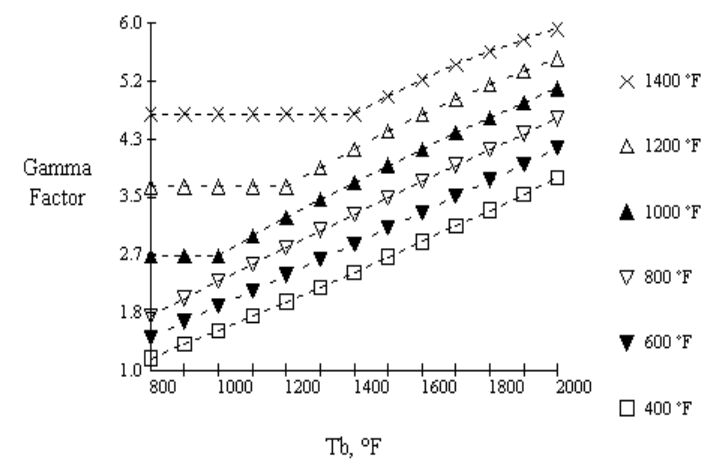
\includegraphics[scale=0.45]{images/gamma}
\caption[Factor de radiación externo]{Factor de radiación externo. Este gráfico requiere de la temperatura promedio del gas y de la temperatura promedio de la superficie del tubo.}
\label{fig:gamma}
\end{center}
\end{figure}

\section{Métodos aproximados}
\par A modo de referencia se describen los métodos utilizados a continuación, ya que serán nombrados mas adelante.

\subsection{Newton Raphson}
\par Es un algoritmo para encontrar aproximaciones de los ceros o raíces de una función real. También puede ser usado para encontrar el máximo o mínimo de una función, encontrando los ceros de su primera derivada, pero nuestro caso de enfoque será el mencionado inicialmente.

\par El método de Newton es un método abierto, en el sentido de que no está garantizada su convergencia global. La única manera de alcanzar la convergencia es seleccionar un valor inicial (semilla) lo suficientemente cercano a la raíz buscada. Así, se ha de comenzar la iteración con un valor razonablemente cercano al cero (también denominado punto de arranque o valor supuesto). La relativa cercanía del punto inicial a la raíz depende mucho de la naturaleza de la propia función; si ésta presenta múltiples puntos de inflexión o pendientes grandes en el entorno de la raíz, entonces las probabilidades de que el algoritmo diverja aumentan, lo cual exige seleccionar un valor supuesto cercano a la raíz. Una vez que se ha hecho esto, el método linealiza la función por la recta tangente en ese valor supuesto. La abscisa en el origen de dicha recta será, según el método, una mejor aproximación de la raíz que el valor anterior. Se realizarán sucesivas iteraciones hasta que el método haya convergido lo suficiente. 

\par Así como el valor inicial, el paso de cada iteración y la tolerancia, todas son variables que se ajustan a conveniencia en este método; los rangos de operación alcanzados por el simulador del horno dependerán en gran medida de estos valores.

\par La implementación usada puede verse en los anexos donde se encuentra el código fuente del simulador.

\subsection{Bisección}

\par Es también un algoritmo de búsqueda de raíces que trabaja dividiendo un intervalo dado a la mitad y seleccionando el subintervalo que tiene la raíz. Suele requerir más iteraciones para alcanzar la tolerancia deseada que el Newton Raphson descrito anteriormente, además de conocer de antemano el intervalo donde se encuentra la raíz deseada, su ventaja es que en funciones continuas se puede garantizar su convergencia.
\par Se basa en el teorema del valor intermedio (TVI), el cual establece que toda función continua $f$ en un intervalo cerrado $[a,b]$ toma todos los valores que se hallan entre $f(a)$ y $f(b)$. 
Esto es que todo valor entre $f(a)$ y $f(b)$ es la imagen de al menos un valor en el intervalo $[a,b]$. En caso de que $f(a)$ y $f(b)$ tengan signos opuestos, el valor cero sería un valor intermedio entre $f(a)$ y $f(b)$, por lo que con certeza existe un  $p\in [a,b]$ que cumple  $f(p)=0$. 
De esta forma, se asegura la existencia de al menos una solución de la ecuación $f(x)=0$.